\documentclass[12pt,a4paper]{article}
\usepackage[utf8]{vietnam}
\usepackage{amsmath,amssymb,amsfonts}
\usepackage[margin=2cm]{geometry}
\usepackage{fancyhdr}
\usepackage{tikz}
\usepackage{tkz-tab}

\pagestyle{fancy}
\fancyhf{}
\lhead{\textbf{ĐỀ THI KHẢO SÁT CHẤT LƯỢNG TOÁN 12 --- MÃ ĐỀ 209}}
\rhead{\textit{Chủ đề: Khảo sát hàm số}}
\rfoot{\small Trang \thepage}
\lfoot{\small\textit{Integra Typesetter}}
\renewcommand{\headrulewidth}{0.4pt}
\renewcommand{\footrulewidth}{0.4pt}

\newcounter{ex}
\newenvironment{ex}[1][]{%
	\refstepcounter{ex}%
	\par\smallskip\noindent\textbf{Câu \theex.} #1\ignorespaces
}{\par}

\providecommand{\True}{}

\newlength{\widthcha}
\newlength{\widthchb}
\newlength{\widthchc}
\newlength{\widthchd}

\newcommand{\choiceFour}[4]{%
	\par\smallskip
	\noindent\textbf{A.} #1\par
	\noindent\textbf{B.} #2\par
	\noindent\textbf{C.} #3\par
	\noindent\textbf{D.} #4\par\smallskip
}

\newcommand{\choiceTwo}[4]{%
	\ifdim\widthcha<0.46\linewidth
	\ifdim\widthchb<0.46\linewidth
	\ifdim\widthchc<0.46\linewidth
	\ifdim\widthchd<0.46\linewidth
	\par\smallskip\noindent
	\begin{minipage}[t]{0.48\linewidth}\textbf{A.} #1\end{minipage}\hfill
	\begin{minipage}[t]{0.48\linewidth}\textbf{B.} #2\end{minipage}\par\smallskip\noindent
	\begin{minipage}[t]{0.48\linewidth}\textbf{C.} #3\end{minipage}\hfill
	\begin{minipage}[t]{0.48\linewidth}\textbf{D.} #4\end{minipage}\par\smallskip
	\else\choiceFour{#1}{#2}{#3}{#4}\fi
	\else\choiceFour{#1}{#2}{#3}{#4}\fi
	\else\choiceFour{#1}{#2}{#3}{#4}\fi
	\else\choiceFour{#1}{#2}{#3}{#4}\fi
}

\newcommand{\choice}[4]{%
	\settowidth{\widthcha}{\textbf{A.} #1}%
	\settowidth{\widthchb}{\textbf{B.} #2}%
	\settowidth{\widthchc}{\textbf{C.} #3}%
	\settowidth{\widthchd}{\textbf{D.} #4}%
	\ifdim\widthcha<0.22\linewidth
	\ifdim\widthchb<0.22\linewidth
	\ifdim\widthchc<0.22\linewidth
	\ifdim\widthchd<0.22\linewidth
	\par\smallskip\noindent
	\begin{minipage}[t]{0.24\linewidth}\textbf{A.} #1\end{minipage}\hfill
	\begin{minipage}[t]{0.24\linewidth}\textbf{B.} #2\end{minipage}\hfill
	\begin{minipage}[t]{0.24\linewidth}\textbf{C.} #3\end{minipage}\hfill
	\begin{minipage}[t]{0.24\linewidth}\textbf{D.} #4\end{minipage}\par\smallskip
	\else\choiceTwo{#1}{#2}{#3}{#4}\fi
	\else\choiceTwo{#1}{#2}{#3}{#4}\fi
	\else\choiceTwo{#1}{#2}{#3}{#4}\fi
	\else\choiceTwo{#1}{#2}{#3}{#4}\fi
}

\newcommand{\choiceTF}[4]{%
	\par\smallskip
	\noindent\textbf{Đáp án:}\quad a) #1 \qquad b) #2 \qquad c) #3 \qquad d) #4\par\smallskip
}

\newcommand{\shortans}[1]{%
	\par\smallskip
	\noindent\textbf{Đáp số:}\quad \fbox{\textbf{#1}}\par\smallskip
}

\newcommand{\loigiai}[1]{%
	\par\smallskip
	\noindent\textit{\textbf{Lời giải:}}\par
	#1\par\medskip\hrule\medskip
}

\begin{document}

\begin{center}
{\Large \textbf{ĐỀ THI KHẢO SÁT CHẤT LƯỢNG - MÃ ĐỀ 209}} \\[2mm]
\textbf{Môn: Toán - Lớp 12} \\
\textit{Chủ đề: Khảo sát hàm số}
\end{center}
\vspace{2mm}

% PHẦN 1: TRẮC NGHIỆM 4 LỰA CHỌN
\subsection*{Phần 1. Trắc nghiệm nhiều phương án lựa chọn}
\textit{Thí sinh trả lời từ câu 1 đến câu 4. Mỗi câu hỏi thí sinh chỉ chọn một phương án.}

\begin{ex}%[PH1_C2]%[Nhận dạng cực trị từ đồ thị]%[12D1Y2]
Cho hàm số $y = ax^3 + bx^2 + cx + d$ có đồ thị là đường cong trong hình bên. Giá trị cực đại của hàm số đã cho là:
\begin{center}
\begin{tikzpicture}[scale=0.8]
\draw[->] (-2,0) -- (3,0) node[below] {$x$};
\draw[->] (0,-2) -- (0,4) node[left] {$y$};
\node at (0,0) [below left] {$O$};
\draw[domain=-1.2:2.2,smooth,variable=\x,blue,thick] plot (\x,{(\x)^3 - 3*(\x) + 2});
\draw[dashed] (1,0) node[below] {$1$} -- (1,0) -- (1,0);
\draw[dashed] (-1,0) node[below] {$-1$} -- (-1,4);
\end{tikzpicture}
\end{center}
\choice
{$y = 1$.}
{$y = 0$.}
{\True $y = 4$.}
{$y = 2$}
\loigiai{
Từ đồ thị, hàm số đạt cực đại tại điểm $x = -1$ và giá trị cực đại là $y = 4$.
}
\end{ex}

\begin{ex}%[PH1_C4]%[Nhận dạng đồ thị hàm số bậc bốn]%[12D1Y4]
Đồ thị của hàm số nào dưới đây có dạng như đường cong trong hình bên?
\begin{center}
\begin{tikzpicture}[scale=0.7]
\draw[->] (-2,0) -- (2,0) node[below] {$x$};
\draw[->] (0,-1) -- (0,5) node[left] {$y$};
\node at (0,0) [below left] {$O$};
\draw[domain=-1.3:1.3,smooth,variable=\x,blue,thick] plot (\x,{(\x)^4 - 2*(\x)^2 + 3});
\end{tikzpicture}
\end{center}
\choice
{$y = -x^4 + 2x^2 + 3$.}
{$y = x^3 - 3x + 3$.}
{\True $y = x^4 - 2x^2 + 3$.}
{$y = \dfrac{x - 1}{x + 1}$.}
\loigiai{
Đồ thị có dạng của hàm số trùng phương $y = ax^4 + bx^2 + c$ với hệ số $a > 0$ và có 3 điểm cực trị. Do đó chọn $y = x^4 - 2x^2 + 3$.
}
\end{ex}

\begin{ex}%[PH1_C1]%[Đọc hiểu bảng biến thiên]%[12D1Y1]
Cho hàm số $y = f(x)$ có bảng biến thiên như sau:
\begin{center}
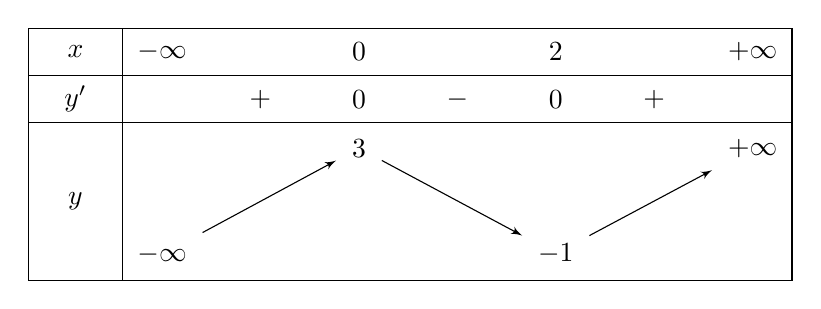
\begin{tikzpicture}
\tkzTabInit[lgt=1.2,espcl=2.5]{$x$/0.6,$y'$/0.6,$y$/2}{$-\infty$,$0$,$2$,$+\infty$}
\tkzTabLine{,+,$0$,-,$0$,+,}
\tkzTabVar{-/ $-\infty$ ,+/$3$,-/$-1$,+/$+\infty$}
\end{tikzpicture}
\end{center}
Hàm số đã cho đồng biến trên khoảng nào dưới đây?
\choice
{$(0; 2)$.}
{$(2; +\infty)$.}
{$(-\infty; 3)$.}
{\True $(-\infty; 0)$.}
\loigiai{
Dựa vào bảng biến thiên, đạo hàm $y' > 0$ trên các khoảng $(-\infty; 0)$ và $(2; +\infty)$. Do đó hàm số đồng biến trên khoảng $(-\infty; 0)$.
}
\end{ex}

\begin{ex}%[PH1_C3]%[Tìm tiệm cận]%[12D1Y3]
Tiệm cận ngang của đồ thị hàm số $y = \dfrac{2x - 1}{x + 1}$ là đường thẳng:
\choice
{$x = -1$.}
{$y = -1$.}
{$x = 2$.}
{\True $y = 2$.}
\loigiai{
Ta có $\lim_{x \to \pm\infty} \dfrac{2x - 1}{x + 1} = 2$. Vậy tiệm cận ngang của đồ thị hàm số là $y = 2$.
}
\end{ex}

% PHẦN 2: ĐÚNG / SAI
\subsection*{Phần 2. Câu trắc nghiệm đúng sai}
\textit{Thí sinh trả lời từ câu 1. Trong mỗi ý a), b), c), d) ở mỗi câu, thí sinh chọn đúng hoặc sai.}

\begin{ex}%[PH2_C1]%[Khảo sát hàm số bậc ba]%[12D1M1]
Cho hàm số $y = x^3 - 3x^2 + 2$. Các mệnh đề sau đây đúng hay sai?
\begin{enumerate}
    \item[a)] Hàm số đồng biến trên khoảng $(0; 2)$.
    \item[b)] Hàm số đạt cực đại tại điểm $x = 0$.
    \item[c)] Giá trị cực tiểu của hàm số bằng $-2$.
    \item[d)] Đồ thị hàm số có tâm đối xứng là điểm $I(1; 0)$.
\end{enumerate}
\choiceTF
{Sai}
{\True Đúng}
{\True Đúng}
{\True Đúng}
\loigiai{
Ta có $y' = 3x^2 - 6x$; $y'' = 6x - 6$.\\
- $y' = 0 \Leftrightarrow x = 0$ hoặc $x = 2$. Bảng biến thiên cho thấy hàm số đồng biến trên $(-\infty; 0)$ và $(2; +\infty)$, nghịch biến trên $(0; 2)$ $\rightarrow$ a Sai.\\
- Hàm số đạt cực đại tại $x = 0$ và $y_{CD} = 2$ $\rightarrow$ b Đúng.\\
- Hàm số đạt cực tiểu tại $x = 2$ và $y_{CT} = 2^3 - 3(2)^2 + 2 = -2$ $\rightarrow$ c Đúng.\\
- Điểm uốn $I(1; 0)$ là tâm đối xứng của đồ thị hàm số $\rightarrow$ d Đúng.
}
\end{ex}

% PHẦN 3: TRẢ LỜI NGẮN
\subsection*{Phần 3. Câu trắc nghiệm trả lời ngắn}
\textit{Thí sinh trả lời từ câu 1 đến câu 2.}

\begin{ex}%[PH3_C1]%[Tìm giá trị lớn nhất nhỏ nhất]%[12D1V1]
Tìm giá trị lớn nhất $M$ của hàm số $y = x^3 - 3x + 2$ trên đoạn $[0; 2]$.
\shortans{4}
\loigiai{
Ta có $y' = 3x^2 - 3$; $y' = 0 \Leftrightarrow x = \pm 1$.\\
Giá trị của hàm số tại các điểm: $f(0) = 2$, $f(1) = 0$, $f(2) = 4$.\\
Vậy giá trị lớn nhất của hàm số trên đoạn $[0; 2]$ bằng $4$.
}
\end{ex}

\begin{ex}%[PH3_C2]%[Tiệm cận và hệ số đồ thị]%[12D1V2]
Cho hàm số $y = \dfrac{ax + b}{x - 1}$ có đồ thị nhận đường thẳng $x = 1$ làm tiệm cận đứng và đường thẳng $y = 2$ làm tiệm cận ngang. Tính giá trị của biểu thức $P = a + b$.
\shortans{2}
\loigiai{
Đồ thị hàm số có tiệm cận đứng $x = 1$ và tiệm cận ngang $y = a = 2$. Suy ra $P = a + b = 2$.
}
\end{ex}

\end{document}
